% Chapter Template

\chapter{State of the art} % Main chapter title

\label{ChapterX} % Change X to a consecutive number; for referencing this chapter elsewhere, use \ref{ChapterX}

%----------------------------------------------------------------------------------------
%	SECTION 1
%----------------------------------------------------------------------------------------

\section{Geospatial analysis in Data Science}

Maps are an increasingly popular way to visualise data where some form of geographic aspect is an important element of the analysis. The website London Mapping (\cite{LMap}) is a good example of the large amount of data analysis and visualisation taking place through the creation of various types of map for the city of London alone.

\begin{figure}[H]
\centering
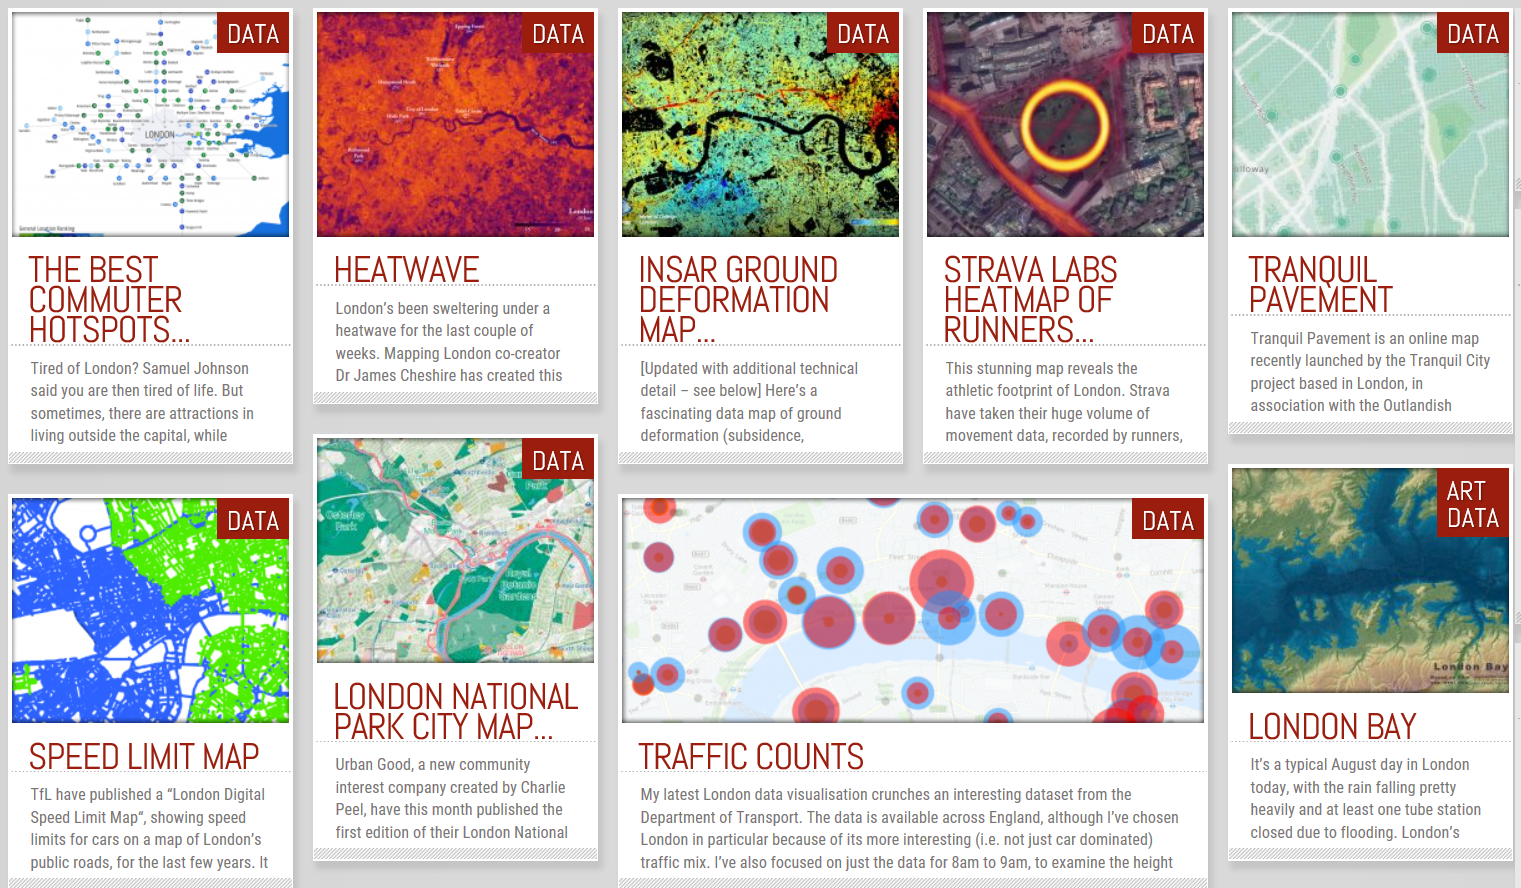
\includegraphics[scale=0.5]{figures/london_mapping}
\decoRule
\caption{An range of the maps exploring London on the Mapping London website. This website has been created by academics from the geography department at UCL and features a range of data-driven maps using various geospatial techniques.}
\end{figure}

There are several reasons why maps a a good choice for data visualisation which include:
\begin{itemize}
\item
They provide a real-world context for the data, helping the audience to understand the analysis
\item
They allow users to compare data over different areas or regions at a glance
\end{itemize}

Data Science techniques play an important role in the creation of this kind of visualisation. Most map visualisations represent locations through coordinate reference systems which represent locations. These locations can be specific locations represented by pairs of coordinates, most often (latitude, longitude), or areas which would be represented by polygons consisting of multiple coordinate pairs. Data Science techniques are required to design functions and algorithms to map, aggregate or disaggregate data between different types of geometry and different coordinate reference systems. 
	
%-----------------------------------
%	SUBSECTION 1
%-----------------------------------
\subsection{Point Maps}
One mapping technique often used in interactive visualisations would be a point map where specific instances of something are plotted as points in the geo-location in which they occur. This form of mapping would use a coordinate pair, often latitude and longditude but potentially an Ordnance Survey grid reference or other coordinate reference system. An example of this would be the Great British Public Toilet Map (\cite{rca14})

\begin{figure}[H]
\centering
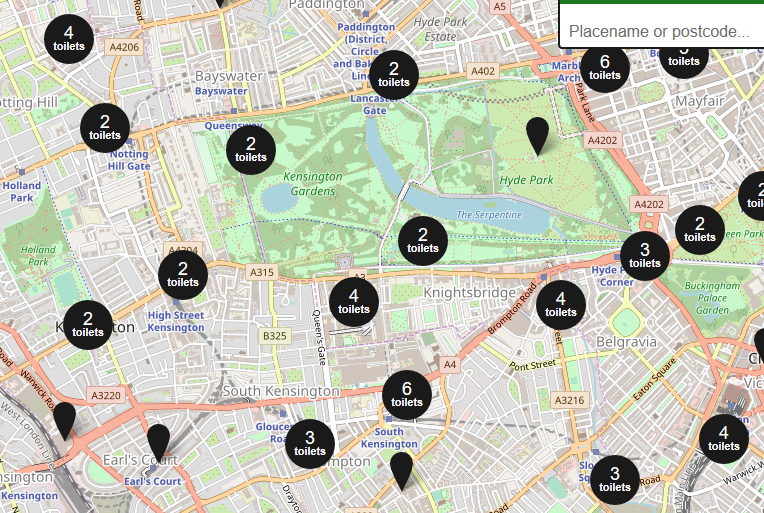
\includegraphics[scale=0.5]{figures/toilets_point}
\decoRule
\caption{An example of a point map - the Great British Public Toilet map created by the Royal College of Art in 2014 showing instances of public lavatories across the country.}
\end{figure}

%-----------------------------------
%	SUBSECTION 2
%-----------------------------------

\subsection{Choropleth Maps}
The city of Toronto is a good example of where an informative interactive well-being map has been created (\cite{toronto_2018}). On this map a user can click on an area and is presented with a panel showing the values for a number of measures.

\begin{figure}[H]
\centering
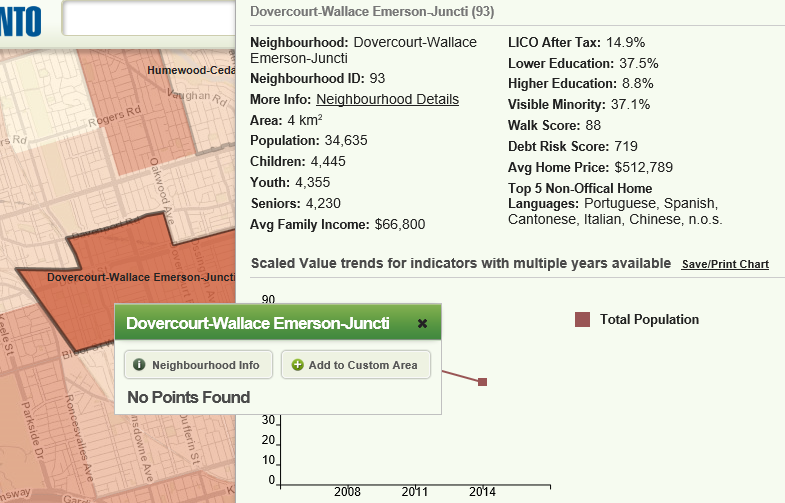
\includegraphics[scale=0.5]{figures/toronto_choropleth}
\decoRule
\caption{An example of a choropleth map - created by the City of Toronto to provide information about the neighbourhoods of urban Toronto.}
\end{figure}

The Toronto map uses a thematic mapping technique known as a Choropleth map, using shape files where polygons represent an area of space, in this instance neighbourhoods, with the colour of the polygon related to the value of the area in question.
This map is an excellent design example for this project as the geometries used, in this case neighbourhoods of Toronto, are of a similar geospatial representation to London Wards. The project map will be based on median house prices and hovering over an area will display the values of the well-being indicators and the projected values of the model.

%-----------------------------------
%	SUBSECTION 3
%-----------------------------------

\subsection{Heat Maps}
Real estate values have also been an area of interest for mapping. In recent times these visual displays of real estate value have often been created by the commercial sector, for example, UK property price maps created by the estate agent Zoopla (\cite{zoopla}). This is an example of a heat map.
Heat maps share similarities with Choropleth maps in that they assign a colour to an area based on the magnitude of a particular value. Where these two types of map differ is that heat maps assign colour to a cluster of connected points whereas for Choropleth maps, the colouration is based on a value for a polygon representing a given area, usually a administrative or political boundary.

\begin{figure}[H]
\centering
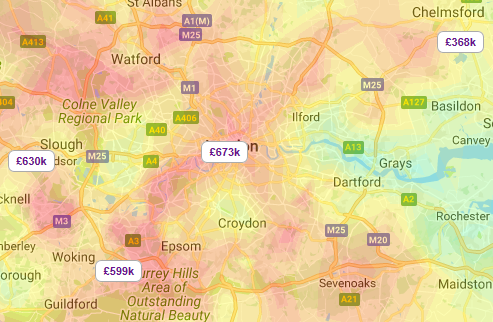
\includegraphics[scale=1]{figures/zoopla_heat}
\decoRule
\caption{An example of a heat map - a 2011 map created by the estate agents Zoopla to show UK average house prices.}
\end{figure}

%-----------------------------------
%	SUBSECTION 4
%-----------------------------------

\subsection{Network Maps}
An interesting alternative approach has been taken by (\cite{QAS16}) who have created a series of interactive maps using crowdsourced data and image processing techniques. The locations used in the maps created by Quercia et al. use specific locations represented by images and sound recordings rather than areas of space. Here, rather than using traditional spatial analysis techniques, the maps have been created using graphs which represent London as a network. The location of the images/sounds are the nodes and the routes between them form the vertices.

\begin{figure}[H]
\centering
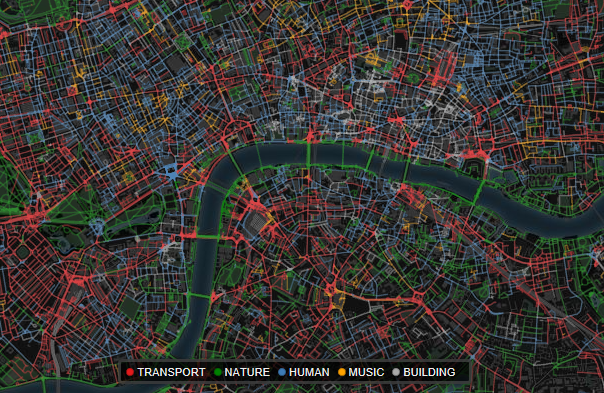
\includegraphics[scale=0.8]{figures/noise_network}
\decoRule
\caption{An example of a network map - created by Quercia, Aiello and Schifanello in 2016, this map categorises each road in London based on the primary type of noise heard in the location.}
\end{figure}


